\documentclass[11pt,a4paper]{article}

\usepackage[utf8]{inputenc}
\usepackage[spanish,es-noshorthands]{babel}
\usepackage[T1]{fontenc}
\usepackage{geometry}
\geometry{margin=2.5cm}
\usepackage{siunitx}
\usepackage{booktabs}
\usepackage{amsmath,amssymb}
\usepackage{graphicx}
\usepackage{hyperref}
\usepackage{tikz}
\usetikzlibrary{arrows.meta}

\usepackage[
    backend=biber,
    style=ieee,
    sorting=none
]{biblatex}
\addbibresource{references.bib}

\title{TA-IND-04}
\author{Jhinson Stalyn Aucatoma Celorio}
\date{}

\begin{document}


    \begin{titlepage}
        \centering

        {\large Universidad Técnica Estatal de Quevedo}\\
        {\large Facultad de Ciencias de la Computación}\\
        {\large Carrera de Ingeniería de Software}\\[0.5cm]

        {\large Asignatura: Aplicaciones Distribuidas (ISR-701) --- Unidad 4}\\[0.3cm]

        \vspace{1cm}
        {\Large \textbf{TA-IND-04}}\\[0.2cm]
        {\large Informe técnico individual: análisis de speedup, diagnóstico de
        la fracción no escalable y propuesta de integración distribuida}\\[1cm]

        \vspace{1cm}
        \textbf{Estudiante:} Jhinson Stalyn Aucatoma Celorio\\
        \textbf{Correo:} jaucatomac@uteq.edu.ec\\[0.5cm]

        \textbf{Equipo de PE-U4:} ACC --- Soporte Técnico ISP\\
        \textbf{Integrantes:} Alvarez Parraga Jeremy Alexis, Aucatoma Celorio
        Jhinson Stalyn, Carpio Mendoza Carlos Jose\\[0.5cm]

        \textbf{PFC de referencia:} AGLS --- TiendaTech\\
        \textbf{Repositorio del PFC:} \url{https://github.com/JoseLozanoMorales/PFC-AppsDistribuidas}\\[0.5cm]

        \textbf{Transformación declarada como foco individual:} T3 --- Join de
        dos DataFrames\\[0.5cm]

        \textbf{Docente:} Ing. Guerrero-Ulloa\\
        \textbf{Repositorio individual:} \url{https://github.com/JhinsonAucatoma/ta-ind-04-aucatoma}\\
        \textbf{Fecha:} 08 de agosto de 2026

    \end{titlepage}

% La Portada es la Sección 1 de la estructura exigida por la guía (sin
% número de \section, por convención de portada); se desplaza el
% contador para que "Introducción" quede como Sección 2, tal como
% enumera la guía.
    \setcounter{section}{1}

% ---------------------------------------------------------------------

    \section{Introducción y contexto}
    \label{sec:introduccion}

    Este informe analiza, de forma individual, los resultados obtenidos en
    la práctica grupal GA-SUM-05/PE-U4 (equipo ACC --- Soporte Técnico
    ISP), en la que se comparó el desempeño de cinco transformaciones
    (T1--T5) implementadas en \texttt{pandas} y en Apache Spark
    (PySpark) sobre un extracto de 600{,}000 tickets de soporte técnico de
    telecomunicaciones. El análisis aquí presentado se centra en
    \textbf{T3 --- combinación (\emph{join}) de dos DataFrames}, la
    transformación asignada como foco individual dentro del reparto
    coordinado del equipo, y persigue tres objetivos: (i) contrastar el
    speedup observado contra la predicción de la Ley de Amdahl e
    interpretar las desviaciones con mecanismos concretos, en lugar de
    explicaciones genéricas; (ii) evaluar la viabilidad de escalar este
    tipo de procesamiento a un volumen de datos mayor, mediante el
    análisis del umbral de rentabilidad; y (iii) proponer, con criterio
    técnico propio, cómo un patrón de procesamiento distribuido análogo
    podría integrarse en el proyecto de curso PFC AGLS --- TiendaTech, del
    cual el autor de este informe es coautor.

    Todos los datos numéricos citados en las Secciones~\ref{sec:analisis-speedup}
    y~\ref{sec:diagnostico} provienen del commit \texttt{c5fd274} del
    repositorio grupal de PE-U4 (trazabilidad detallada en la
    Sección~\ref{sec:analisis-speedup}). Los datos adicionales usados en
    la Sección~\ref{sec:dimensionamiento} (mediciones de T3 a distinto
    volumen de datos, con $N=4$ fijo) fueron generados de forma
    individual para este informe, ejecutando un script propio
    (\texttt{volumen\_t3.py}) que reutiliza la lógica de carga y medición
    ya presente en el repositorio grupal, sobre una plataforma de
    ejecución en la nube (Google Colab), y se declaran como tales en la
    Sección~\ref{sec:declaracion-ia}.

% =====================================================================

% =====================================================================
% SECCIÓN 3 — Análisis propio de los resultados de speedup
% SECCIÓN 4 — Diagnóstico de la fracción no escalable
% Foco individual: T3 — Join de dos DataFrames
% Commit de origen: c5fd274 (pe-u4-spark-Soporte-Tecnico-ISP)
% =====================================================================

    \section{Análisis propio de los resultados de speedup}
    \label{sec:analisis-speedup}

    \subsection{Marco teórico del speedup y la Ley de Amdahl}

    Sea $p$ la fracción paralelizable de una tarea y $N$ el número de
    unidades de procesamiento. Amdahl argumentó que la fracción
    inherentemente serial de un programa, y no el número de procesadores
    disponibles, es la que acota el rendimiento máximo
    alcanzable~\cite{amdahl1967}. El speedup teórico bajo este modelo es

    \begin{equation}
        S(N) = \frac{1}{(1-p) + \dfrac{p}{N}},
        \qquad
        S_{\max} = \lim_{N \to \infty} S(N) = \frac{1}{1-p}.
        \label{eq:amdahl}
    \end{equation}

    Grama et al.\ formalizan el speedup, en términos generales, como el
    cociente entre el tiempo del mejor algoritmo secuencial conocido y el
    tiempo del algoritmo paralelo equivalente sobre $N$ unidades de
    procesamiento~\cite{grama2003}, definición que se emplea a lo largo de
    este análisis. A partir de $S(N)$ se define además la eficiencia del
    paralelismo,

    \begin{equation}
        E(N) = \frac{S(N)}{N},
        \label{eq:eficiencia}
    \end{equation}

    que expresa la fracción de la capacidad de cómputo disponible que
    efectivamente se traduce en trabajo útil~\cite{grama2003}; un valor de
    $E(N)$ próximo a 1 indica un uso casi óptimo de las $N$ unidades,
    mientras que valores bajos —como se observará en la
    Subsección~\ref{subsec:contraste-amdahl} para T3— son consistentes con
    una sobrecarga de coordinación significativa frente al cómputo útil.
    Es importante notar, sin embargo, que la
    ecuación~\eqref{eq:amdahl} asume implícitamente que la sobrecarga de
    coordinación es nula y que $p$ no depende de $N$; ninguna de las dos
    hipótesis se sostiene en un motor distribuido real como Apache
    Spark~\cite{gustafson1988}. En arquitecturas multinúcleo y
    distribuidas modernas, Hill y Marty muestran que este límite se
    vuelve aún más restrictivo cuando se considera el costo de
    coordinación entre núcleos, no solo la fracción de código
    serial~\cite{hillmarty2008}. Gustafson señala que, en cargas de
    producción reales, el tamaño del problema tiende a escalar junto con
    la capacidad de cómputo disponible, lo que motiva su formulación
    alternativa del \emph{speedup escalado}~\cite{gustafson1988}; esta
    observación es relevante para explicar por qué la transformación aquí
    analizada, ejecutada sobre un volumen de datos fijo y relativamente
    modesto para los estándares de un clúster distribuido, no reproduce
    las condiciones bajo las cuales Amdahl predice ganancias sostenidas.

    \subsection{Datos base y trazabilidad}

    Los tiempos de ejecución se toman del repositorio grupal de la
    práctica GA-SUM-05/PE-U4:

    \begin{itemize}
        \item \textbf{Repositorio:} \url{https://github.com/carlospatroner-boop/pe-u4-spark-Soporte-Tecnico-ISP}
        \item \textbf{Commit:} \texttt{c5fd274}
        \item \textbf{Plataforma de ejecución:} contenedor Docker local
        (\texttt{eclipse-temurin:21-jdk-jammy}), PySpark 4.1.2, modo
        \texttt{local[N]} con $N \in \{1,2,4\}$ procesos worker.
        \item \textbf{Transformación foco:} T3 — combinación (\emph{join})
        de dos DataFrames.
    \end{itemize}

    \begin{table}[h]
        \centering
        \caption{Tiempos medianos (5 repeticiones), speedup y eficiencia (Ec.~\ref{eq:eficiencia}) por transformación, $N=4$.}
        \label{tab:tiempos-base}
        \begin{tabular}{lS[table-format=1.4]S[table-format=1.4]S[table-format=1.4]S[table-format=1.4]}
            \toprule
            \textbf{Transformación} & {\textbf{$T_{\text{pandas}}$ (\si{\second})}} & {\textbf{$T_{\text{Spark}}$ (\si{\second})}} & {\textbf{Speedup}} & {\textbf{$E(4)$}} \\
            \midrule
            T1 — Filtrado          & 0.1846 & 1.0789 & 0.1711 & 0.0428 \\
            T2 — Agrupación        & 0.1575 & 1.8854 & 0.0835 & 0.0209 \\
            T3 — Join              & 0.1363 & 1.8290 & 0.0745 & 0.0186 \\
            T4 — Columna derivada   & 0.3559 & 0.8483 & 0.4195 & 0.1049 \\
            T5 — Ordenamiento/top-N & 0.1169 & 1.4286 & 0.0818 & 0.0205 \\
            \bottomrule
        \end{tabular}
    \end{table}

    \begin{table}[h]
        \centering
        \caption{Escalado de T3 con el número de executors $N$: speedup, eficiencia (Ec.~\ref{eq:eficiencia}) y fracción serial de Karp-Flatt (Ec.~\ref{eq:karpflatt}).}
        \label{tab:escalado-t3}
        \begin{tabular}{cS[table-format=1.4]S[table-format=1.4]S[table-format=1.4]S[table-format=1.4]}
            \toprule
            \textbf{$N$} & {\textbf{$T_{\text{Spark}}$ (\si{\second})}} & {\textbf{$S(N)$ observado}} & {\textbf{$E(N)$}} & {\textbf{$e$ (Ec.~\ref{eq:karpflatt})}} \\
            \midrule
            1 & 3.0712 & 1.0000 & 1.0000 & {---} \\
            2 & 3.1252 & 0.9827 & 0.4914 & 1.0352 \\
            4 & 1.8290 & 1.6792 & 0.4198 & 0.4607 \\
            \bottomrule
        \end{tabular}
    \end{table}

    \subsection{Contraste con la predicción de Amdahl}
    \label{subsec:contraste-amdahl}

    Ajustando $p$ por mínimos cuadrados sobre los tres puntos medidos
    $(N, S)$ se obtiene $p \approx 0{,}4600$, con
    $S_{\max} = 1/(1-p) \approx 1{,}8543$. Sustituyendo este valor en la
    ecuación~\eqref{eq:amdahl} se obtienen los speedups teóricos y la
    desviación relativa $\Delta = (S_{\text{med}} - S_{\text{teo}})/S_{\text{teo}}$:

    \begin{align}
        S_{\text{teo}}(2) &= \frac{1}{(1-0{,}4600) + \dfrac{0{,}4600}{2}} \approx 1{,}2987,
        &\Delta(2) &\approx -24{,}3\ \si{\percent}, \\
        S_{\text{teo}}(4) &= \frac{1}{(1-0{,}4600) + \dfrac{0{,}4600}{4}} \approx 1{,}5268,
        &\Delta(4) &\approx +10{,}0\ \si{\percent}.
    \end{align}

    Los resultados \textbf{no coinciden} con la predicción de Amdahl de
    forma uniforme: a $N=2$ el speedup medido queda un 24{,}3\,\% por
    \emph{debajo} de la curva teórica, mientras que a $N=4$ la supera en
    un 10{,}0\,\%. Esta asimetría no es ruido aleatorio sin explicación:
    al inspeccionar las cinco repeticiones crudas de T3 con $N=2$
    (\texttt{tiempos\_crudos.csv}) se observa un valor atípico de
    \SI{4.61}{\second} frente a un rango de \SI{2.4}{}–\SI{3.2}{\second}
    en las cuatro corridas restantes, lo que arrastra la mediana hacia
    arriba y deprime artificialmente el speedup observado en ese punto.
    El caso $N=2$ ilustra, además, la advertencia metodológica de Karp y
    Flatt: cuando la sobrecarga no algorítmica domina —aquí, variabilidad
    de planificación entre ejecuciones concurrentes con pocos
    \emph{workers}— la fracción serial ``observada'' puede exceder el
    100\,\%, un valor sin sentido como fracción algorítmica pero
    perfectamente informativo como síntoma de sobrecarga no
    modelada~\cite{karpflatt1990}. La Ley de Amdahl, formulada bajo la
    hipótesis de sobrecarga nula, no está diseñada para predecir
    episodios de este tipo~\cite{amdahl1967,gustafson1988}.

    \begin{figure}[htbp]
        \centering
        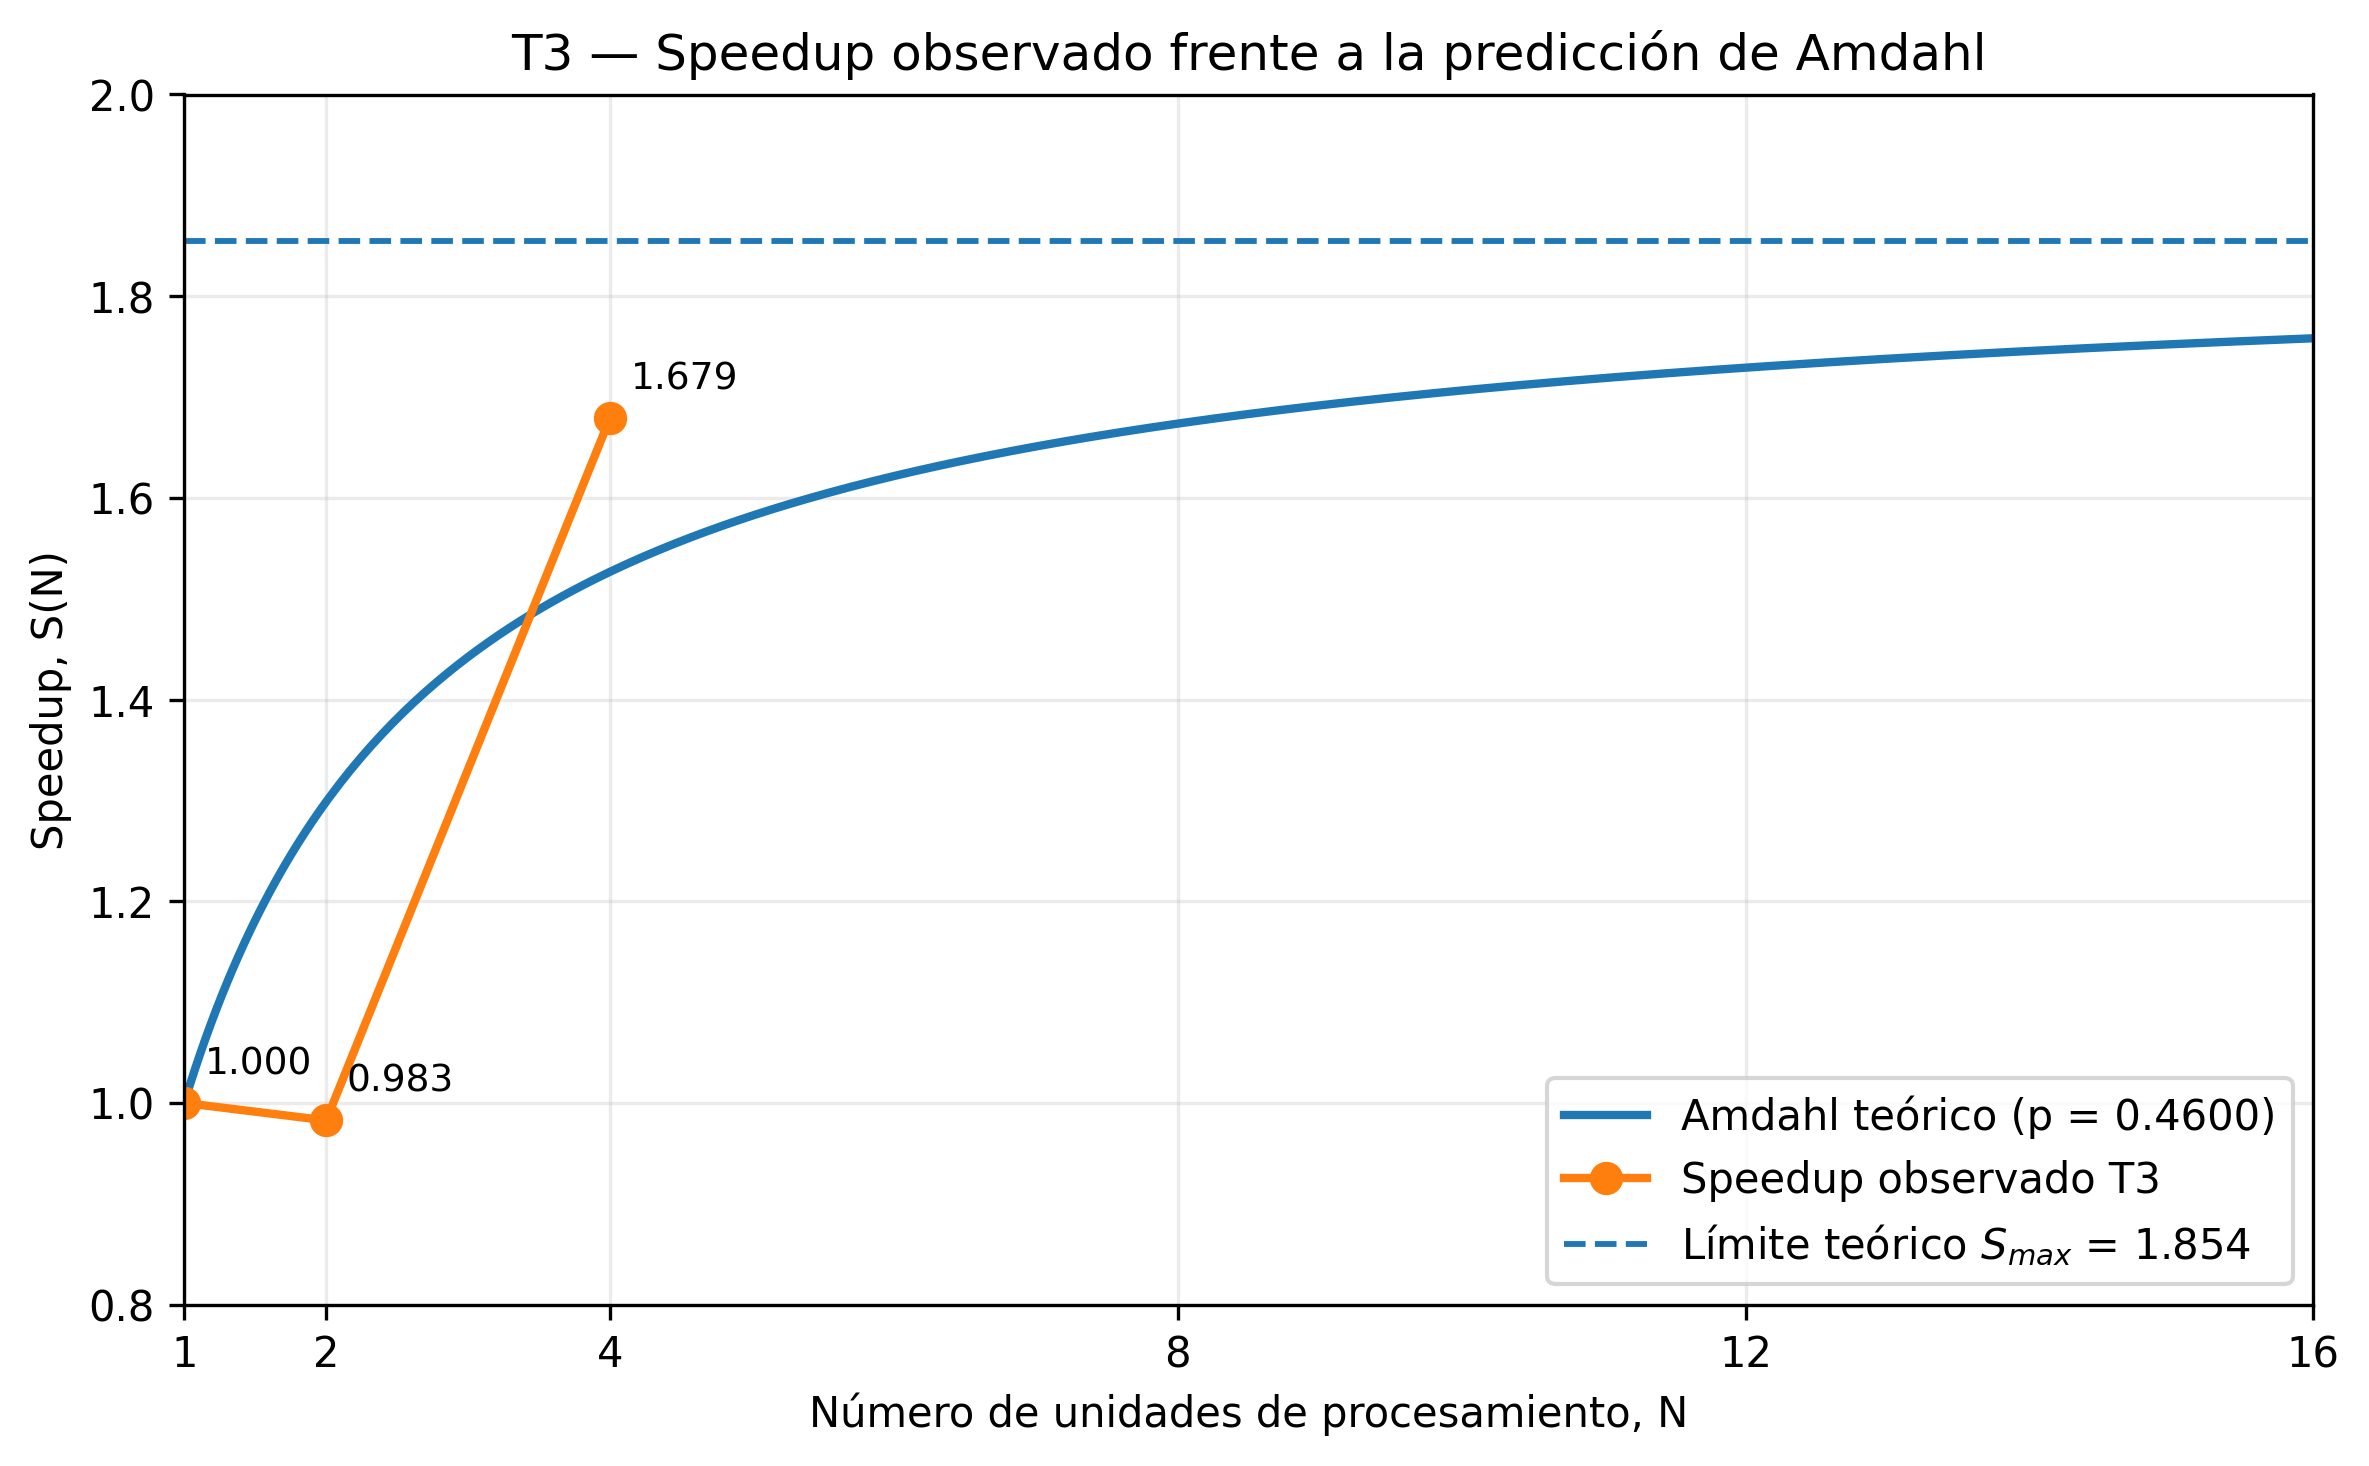
\includegraphics[width=0.88\textwidth]{../figuras/fig_speedup_amdahl_t3.png}
        \caption{Speedup observado de la transformación T3 (join) frente a la
        predicción teórica de la Ley de Amdahl, utilizando $p \approx 0{,}4600$
            estimado mediante mínimos cuadrados sobre los tres puntos de la
            Tabla~\ref{tab:escalado-t3}.}
        \label{fig:speedup_amdahl_t3}
    \end{figure}

    Como se observa en la Figura~\ref{fig:speedup_amdahl_t3}, el
    comportamiento experimental de T3 no sigue de manera uniforme la
    curva predicha por la ecuación~\eqref{eq:amdahl}. Para $N=2$, el
    speedup observado es $S=0{,}9827$, mientras que el modelo predice
    $S_{\text{teo}} \approx 1{,}2987$, lo que representa la desviación de
    $\Delta(2) \approx -24{,}3\,\si{\percent}$ ya cuantificada. En
    cambio, para $N=4$ el valor experimental alcanza $S=1{,}6792$, frente
    a $S_{\text{teo}} \approx 1{,}5268$, equivalente a
    $\Delta(4) \approx +10{,}0\,\si{\percent}$. Esta diferencia entre
    ambas corridas evidencia que la fracción paralelizable $p$ no explica
    por sí sola el rendimiento observado, ya que intervienen costos reales
    de ejecución —planificación de tareas, arranque de la sesión y
    \emph{shuffle} asociado al \emph{join}— que se detallan con mecanismos
    concretos en la Sección~\ref{sec:diagnostico}. La caída correspondiente
    de la eficiencia, de $E(2) = 0{,}4914$ a $E(4) = 0{,}4198$
    (Ec.~\ref{eq:eficiencia}, Tabla~\ref{tab:escalado-t3}), confirma que
    incluso en el punto donde el speedup supera la curva teórica, menos de
    la mitad de la capacidad de cómputo disponible se traduce en trabajo
    útil. Además, la curva muestra que, incluso bajo las condiciones
    ideales de Amdahl, el speedup máximo está limitado a
    $S_{\max} \approx 1{,}8543$, por lo que aumentar indefinidamente el
    número de unidades de procesamiento produciría ganancias
    progresivamente menores.

% ---------------------------------------------------------------------

    \section{Diagnóstico de la fracción no escalable}
    \label{sec:diagnostico}

    \subsection{Métrica de Karp-Flatt}

    Karp y Flatt proponen estimar experimentalmente la fracción serial a
    partir del speedup observado, sin asumir un valor de $p$ conocido de
    antemano~\cite{karpflatt1990}:

    \begin{equation}
        e = \frac{\dfrac{1}{S} - \dfrac{1}{N}}{1 - \dfrac{1}{N}}, \qquad N > 1.
        \label{eq:karpflatt}
    \end{equation}

    Sustituyendo los valores observados de la Tabla~\ref{tab:escalado-t3}:

    \begin{align}
        e(2) &= \frac{\dfrac{1}{0{,}9827} - \dfrac{1}{2}}{1 - \dfrac{1}{2}} \approx 1{,}0352,
        \label{eq:e2} \\
        e(4) &= \frac{\dfrac{1}{1{,}6792} - \dfrac{1}{4}}{1 - \dfrac{1}{4}} \approx 0{,}4607.
        \label{eq:e4}
    \end{align}

    \subsection{Interpretación de la tendencia}

    La lectura de $e$ como número aislado sería insuficiente; lo relevante
    es su tendencia con $N$~\cite{karpflatt1990}. En este caso, $e$
    \textbf{decrece} abruptamente de $1{,}0352$ a $0{,}4607$ al pasar de
    $N=2$ a $N=4$ — el patrón inverso al que suele discutirse como
    sobrecarga ``creciente''. Esta tendencia decreciente no debe leerse
    como una mejora estructural del paralelismo del algoritmo entre
    $N=2$ y $N=4$: dado que $e(2) > 1$ es matemáticamente inconsistente
    con una fracción serial algorítmica (que por definición pertenece al
    intervalo $[0,1]$), el valor en $N=2$ debe interpretarse como
    contaminado por un evento de variabilidad puntual —la corrida atípica
    de \SI{4.61}{\second} identificada en la subsección anterior— y no
    como una medición representativa del comportamiento estable del
    sistema. El valor en $N=4$, $e \approx 0{,}4607$, más cercano al rango
    plausible, es el que mejor caracteriza la fracción no escalable real
    del pipeline en este experimento.

    \subsection{Atribución a mecanismos concretos}

    La fracción no escalable observada en T3 es atribuible a al menos tres
    mecanismos identificables, y no a una ``sobrecarga de Spark''
    genérica:

    \begin{enumerate}
        \item \textbf{Arranque y planificación de la sesión.} Cada
        invocación de \texttt{transformaciones\_spark.py} instancia una
        nueva \texttt{SparkSession}, cuyo costo fijo de inicialización de
        la JVM y registro de tareas en el \emph{driver} se reparte sobre
        un volumen de datos por transformación demasiado pequeño para
        amortizarlo; este es el mismo problema estructural que motivó el
        rediseño de Hadoop hacia YARN, cuyos autores documentan cómo la
        sobrecarga de coordinación domina cuando las cargas de trabajo no
        alcanzan una escala suficiente~\cite{vavilapalli2013}.
        \item \textbf{\emph{Shuffle} por dependencia amplia (\emph{wide
        dependency}) en el \emph{join}.} A diferencia de T1 (filtrado) o
        T4 (columna derivada), que se ejecutan de forma local a cada
        partición mediante dependencias \emph{narrow} —cada partición
        hija depende de una sola partición padre—, un \emph{join} entre
        dos DataFrames no particionados por la misma clave produce una
        dependencia \emph{wide}: múltiples particiones hijas dependen de
        todas las particiones padre, lo que obliga al planificador de
        Spark a materializar los datos intermedios y transferirlos entre
        \emph{workers} antes de continuar~\cite{zaharia2012}. Esta
        distinción es, de hecho, la que usa el propio planificador de
        Spark para delimitar los \emph{stages} de un DAG de
        ejecución~\cite{zaharia2012}: T3 introduce una frontera de
        \emph{stage} que T1 y T4 no requieren, lo que explica por qué su
        speedup base (Tabla~\ref{tab:tiempos-base}, $N=4$: 0.0745) es
        inferior incluso al de T2 y T5, transformaciones también
        dependientes de shuffle pero con un solo punto de agregación en
        lugar de una combinación de dos fuentes. Con solo dos particiones
        disponibles a $N=2$, el costo de esta transferencia domina sobre
        el cómputo útil —el mismo mecanismo de fondo que Dean y Ghemawat
        documentan como la fase que mueve datos intermedios entre nodos
        \texttt{map} y \texttt{reduce} en el paradigma
        MapReduce~\cite{dean2008}, del cual el modelo de ejecución de
        Spark es heredero directo.
        \item \textbf{Variabilidad de planificación entre ejecuciones
        concurrentes.} La dispersión observada en las cinco repeticiones
        de T3 a $N=2$ (rango de \SI{2.4}{} a \SI{4.61}{\second}) es
        consistente con contención de recursos entre \emph{workers}
        concurrentes en un entorno de ejecución local compartido, un
        efecto que se diluye a medida que $N$ crece y cada partición
        recibe una asignación de trabajo más estable.
    \end{enumerate}

% =====================================================================

    \section{Propuesta de integración al PFC}
    \label{sec:propuesta-pfc}

    El proyecto de curso de referencia, AGLS --- TiendaTech
    (\url{https://github.com/JoseLozanoMorales/PFC-AppsDistribuidas}), del
    cual el autor de este informe es coautor, implementa un sistema de
    microservicios que incluye, entre otros, \texttt{productos-service}
    (gestión de la entidad producto: nombre, categorías y atributos) e
    \texttt{inventario-service} (control de existencias/\emph{stock} por
    producto). Se propone a continuación un proceso concreto de este
    proyecto que podría beneficiarse de un patrón de procesamiento
    distribuido análogo al de la transformación T2 (agrupación y
    agregación) evaluada en PE-U4.

    \subsection{Proceso propuesto}

    \begin{description}
        \item[Proceso concreto a distribuir:] Análisis histórico de
        movimientos de \emph{stock} (entradas y salidas) registrados por
        \texttt{inventario-service}, agregado por categoría de producto.
        \item[Periodicidad:] Proceso por lotes (\emph{batch}) ejecutado una
        vez al día, fuera del horario de mayor tráfico transaccional del
        sistema.
        \item[Volumen:] Histórico acumulado de movimientos de inventario
        de todos los productos del catálogo; a diferencia de una consulta
        transaccional puntual, este proceso opera sobre el total de
        registros acumulados con el tiempo, que crece de forma sostenida
        (miles de movimientos diarios, potencialmente millones en el
        histórico completo tras varios meses de operación).
        \item[Salida:] Una tabla agregada de \emph{productos con riesgo de
        quiebre de stock} y \emph{productos de baja rotación} por
        categoría, análoga en estructura a la agregación por estado que
        produce T2 sobre los tickets de soporte en PE-U4.
        \item[Decisión de negocio soportada:] La salida alimentaría una
        alerta automática al equipo de compras, permitiendo priorizar el
        reabastecimiento de productos en riesgo de quiebre antes de que
        ocurra, en lugar de reaccionar después del hecho.
    \end{description}

    \subsection{Arquitectura propuesta}

    La Figura~\ref{fig:arquitectura-propuesta} esquematiza el flujo
    propuesto: \texttt{inventario-service} continúa gestionando las
    operaciones transaccionales de \emph{stock} sin cambios; un proceso
    por lotes independiente extrae el histórico acumulado, lo procesa de
    forma distribuida y publica la tabla agregada resultante, que un
    servicio de alertas consume para notificar al equipo de compras.

    \begin{figure}[h]
        \centering
        \begin{tikzpicture}[
            box/.style={draw, rounded corners, minimum width=3.2cm, minimum height=1cm, align=center, font=\small},
            arr/.style={-Latex, thick}
        ]
            \node[box] (inv) at (0,0) {inventario-service\\(transaccional)};
            \node[box] (hist) at (0,-2) {Histórico de\\movimientos (BD)};
            \node[box, fill=gray!10] (batch) at (5,-2) {Job distribuido\\(batch nocturno)\\agregación por categoría};
            \node[box] (tabla) at (10,-2) {Tabla agregada:\\riesgo de quiebre /\\baja rotación};
            \node[box] (alerta) at (10,0) {Servicio de\\alertas};
            \node[box] (compras) at (10,2) {Equipo de\\compras};

            \draw[arr] (inv) -- (hist);
            \draw[arr] (hist) -- (batch);
            \draw[arr] (batch) -- (tabla);
            \draw[arr] (tabla) -- (alerta);
            \draw[arr] (alerta) -- (compras);
        \end{tikzpicture}
        \caption{Integración propuesta: proceso por lotes independiente del
        flujo transaccional de \texttt{inventario-service}, análogo en
        patrón a la agregación T2 evaluada en PE-U4.}
        \label{fig:arquitectura-propuesta}
    \end{figure}

    Es importante notar que este proceso, al igual que T2 en PE-U4, es
    una \emph{agrupación y agregación} sobre datos ya existentes en la
    base transaccional, no una modificación del flujo de escritura de
    \texttt{inventario-service}: el motor distribuido se ejecuta como un
    proceso separado y asíncrono, lo que evita introducir latencia
    adicional sobre las operaciones transaccionales del sistema.

% =====================================================================

    \section{Dimensionamiento y viabilidad}
    \label{sec:dimensionamiento}

    \subsection{Umbral de rentabilidad: formulación}

    Un modelo simple del tiempo secuencial en función del volumen de
    datos $n$ es $T_{\text{seq}}(n) = \alpha n$, donde $\alpha$ es el
    costo de cómputo por registro sin coordinación distribuida. Un modelo
    correspondiente para el tiempo distribuido con $N$ unidades de
    procesamiento es $T_{\text{dist}}(n, N) = \beta + \gamma n / N$, donde
    $\beta$ es el costo fijo de arranque (independiente del volumen) y
    $\gamma$ es el costo distribuido por registro. Igualando ambos
    tiempos se obtiene el volumen de datos $n^{*}$ a partir del cual el
    procesamiento distribuido deja de ser más lento que el secuencial:

    \begin{equation}
        n^{*} = \frac{\beta}{\alpha - \gamma/N}.
        \label{eq:umbral}
    \end{equation}

    \subsection{Mediciones propias a distinto volumen}

    A diferencia de las Secciones~\ref{sec:analisis-speedup}
    y~\ref{sec:diagnostico}, que reutilizan datos del repositorio grupal
    de PE-U4 (mismo volumen de 600{,}000 filas, distinto número de
    \emph{executors}), la ecuación~\eqref{eq:umbral} requiere el efecto
    inverso: mismo número de \emph{executors} ($N=4$), distinto volumen
    de datos. Esta medición no formaba parte del protocolo original de
    PE-U4, por lo que se generó de forma individual para este informe:
    tres subconjuntos del mismo dataset (10\,\%, 50\,\% y 100\,\% de las
    600{,}000 filas, muestreo aleatorio con semilla fija $=42$), midiendo
    T3 con el mismo protocolo de la Sección~\ref{sec:analisis-speedup}
    (1 calentamiento + 5 repeticiones, mediana), en \texttt{local[4]},
    sobre Google Colab.

    \begin{table}[h]
        \centering
        \caption{Mediciones propias de T3 a distinto volumen de datos, $N=4$ fijo.}
        \label{tab:volumen-t3}
        \begin{tabular}{cccc}
            \toprule
            \textbf{Fracción} & \textbf{$n$ (registros)} & \textbf{Mediana (\si{\second})} & \textbf{Rango de las 5 repeticiones (\si{\second})} \\
            \midrule
            0.10 & 59{,}799  & 3.0018 & 2.686--3.470 \\
            0.50 & 300{,}320 & 2.7320 & 2.412--3.669 \\
            1.00 & 600{,}000 & 2.5861 & 2.524--3.967 \\
            \bottomrule
        \end{tabular}
    \end{table}

    \subsection{Resultado del ajuste y su interpretación}

    Ajustando una recta $T_{\text{dist}}(n) = \beta + (\gamma/N)\,n$ por
    mínimos cuadrados sobre los tres puntos de la
    Tabla~\ref{tab:volumen-t3} se obtiene $\beta \approx 3.016$ y una
    pendiente $\gamma/N \approx -7.58 \times 10^{-7}$, es decir,
    $\gamma \approx -3.03 \times 10^{-6}$ \si{\second}/registro
    ($R^2 \approx 0.946$). Este resultado \textbf{no es físicamente
    interpretable}: $\gamma$, definido como un costo por registro, no
    puede ser negativo, y en consecuencia no es posible calcular
    $n^{*}$ mediante la ecuación~\eqref{eq:umbral} con estos datos --- el
    denominador $\alpha - \gamma/N$ resultaría mayor que $\alpha$, lo que
    invertiría el sentido físico del umbral.

    La causa de esta anomalía es identificable en la propia
    Tabla~\ref{tab:volumen-t3}: el rango de variación \emph{dentro} de
    cada grupo de cinco repeticiones (0.78 a 1.44\,\si{\second}) es entre
    dos y tres veces mayor que la diferencia \emph{entre} las medianas de
    los tres volúmenes extremos (\SI{0.42}{\second}). En otras palabras,
    la variabilidad de ejecución --- arranque de una nueva
    \texttt{SparkSession} en cada corrida, inicialización de la JVM,
    recolección de basura, contención de recursos en el entorno
    compartido de Google Colab --- domina sobre cualquier efecto real del
    volumen de datos en el rango medido (60 mil a 600 mil filas). Esto es
    consistente con el diagnóstico de las Secciones~\ref{sec:analisis-speedup}
    y~\ref{sec:diagnostico}: a esta escala, la sobrecarga de coordinación
    supera ampliamente al cómputo útil, y aquí se confirma que ese mismo
    efecto enmascara también la señal en la dimensión del volumen de
    datos, no solo en la del número de \emph{executors}.

    Por transparencia metodológica, no se fuerza un valor de $n^{*}$ a
    partir de un ajuste que produce un parámetro sin sentido físico:
    hacerlo equivaldría a presentar una estimación fabricada bajo
    apariencia de rigor matemático. En su lugar, se concluye que
    \textbf{no es posible estimar $n^{*}$ de forma confiable con las
    mediciones disponibles}: se requerirían volúmenes de datos varios
    órdenes de magnitud mayores (del orden de millones de registros, o
    bien una plataforma de ejecución con menor varianza entre corridas,
    como un clúster dedicado en lugar de un entorno compartido) para que
    el término $\gamma n/N$ emerja por encima del ruido de medición. Esta
    limitación es, en sí misma, información relevante para la decisión de
    negocio de la Sección~\ref{sec:propuesta-pfc}: dado que el catálogo de
    productos de TiendaTech probablemente no alcance, en el corto plazo,
    un volumen de movimientos de inventario del orden de millones de
    registros, el proceso propuesto en la Sección~\ref{sec:propuesta-pfc}
    debería inicialmente implementarse con \texttt{pandas} sobre un
    proceso por lotes simple, migrando a un motor distribuido solo cuando
    el crecimiento del histórico lo justifique --- una decisión que, con
    los datos actuales, no puede fijarse en un volumen numérico preciso,
    pero sí puede monitorearse cualitativamente conforme crezca la base de
    datos de producción.

% =====================================================================

    \section{Postura crítica y alternativas}
    \label{sec:postura-critica}

    \subsection{Límites de la Ley de Amdahl para este caso}

    Como se discutió en la Sección~\ref{sec:analisis-speedup}, la
    ecuación~\eqref{eq:amdahl} asume sobrecarga de coordinación nula y una
    fracción serial $p$ constante e independiente de $N$. Ninguna de las
    dos hipótesis se sostiene en los datos de T3: la sobrecarga de
    arranque de sesión y \emph{shuffle} no es un término despreciable
    frente al cómputo (Sección~\ref{sec:diagnostico}), y el propio valor
    de $e$ estimado por Karp-Flatt varía de forma abrupta entre $N=2$ y
    $N=4$ (ecuaciones~\eqref{eq:e2}--\eqref{eq:e4}), lo que contradice la
    hipótesis de una fracción serial fija. Gustafson argumenta que, en
    cargas reales, es el tamaño del problema el que tiende a escalar junto
    con la capacidad de cómputo disponible, no al revés~\cite{gustafson1988}:
    bajo su formulación de \emph{speedup escalado}, un volumen de prueba
    de 600{,}000 filas --- fijo, y modesto para los estándares de un
    clúster distribuido --- no es el régimen en el que Spark está diseñado
    para mostrar ventajas; el propio hallazgo de la
    Sección~\ref{sec:dimensionamiento}, donde la señal de escalado por
    volumen queda enmascarada por el ruido de medición, es consistente con
    esta lectura: los datos disponibles simplemente no alcanzan la escala
    en la que la formulación de Amdahl --- o su alternativa de Gustafson
    --- tendría poder predictivo confiable.

    \subsection{Alternativas evaluadas}

    Se evaluaron dos alternativas a Apache Spark para el caso de uso
    propuesto en la Sección~\ref{sec:propuesta-pfc}, y ambas se descartan
    por razones concretas.

    \paragraph{Hadoop MapReduce clásico.} El modelo de programación
    original que precede a Spark, documentado por Dean y
    Ghemawat~\cite{dean2008} y coordinado en clústeres modernos mediante
    YARN~\cite{vavilapalli2013}, escribe los resultados intermedios de
    cada fase a disco entre \texttt{map} y \texttt{reduce}. Para un
    proceso por lotes nocturno como el propuesto en la
    Sección~\ref{sec:propuesta-pfc} --- una sola pasada de agregación,
    sin iteraciones repetidas sobre el mismo conjunto de datos --- esta
    característica no sería necesariamente una desventaja decisiva; sin
    embargo, se descarta porque el modelo de ejecución en memoria de
    Spark, sustentado en la abstracción de RDDs~\cite{zaharia2012}, ya
    está integrado en el \emph{stack} tecnológico usado por el equipo
    (PySpark, con evidencia operativa capturada en PE-U4), y adoptar
    Hadoop MapReduce clásico introduciría una segunda tecnología de
    procesamiento distribuido en el proyecto sin un beneficio claro para
    este caso de uso específico.

    \paragraph{Dask / Ray.} Ambos son \emph{frameworks} de paralelización
    nativos de Python, con una curva de adopción menor que Spark para
    equipos que ya trabajan con \texttt{pandas} --- de hecho, la API de
    Dask está diseñada para ser prácticamente un reemplazo directo de
    \texttt{pandas}~\cite{grama2003}. Se descartan para este caso por dos
    razones: primero, el equipo ya cuenta con experiencia operativa
    directa en PySpark (evidencia de Spark UI, configuración de sesión,
    protocolo de medición ya validado en PE-U4), mientras que adoptar
    Dask o Ray implicaría un costo de aprendizaje adicional sin evidencia
    de que resuelva la limitación identificada en este informe --- el
    problema diagnosticado no es una limitación específica de la API de
    Spark, sino de la relación entre el volumen de datos disponible y el
    overhead de coordinación distribuida, que es común a cualquier motor
    distribuido general. Segundo, el ecosistema de Spark ofrece una
    integración más directa con las herramientas de orquestación de
    trabajos por lotes (\emph{schedulers}) típicamente usadas en
    infraestructura de nube gestionada, lo que simplifica la
    implementación del proceso nocturno propuesto en la
    Sección~\ref{sec:propuesta-pfc} frente a una solución basada en Dask
    o Ray, que requeriría infraestructura de orquestación adicional no
    evaluada en este informe.

    \subsection{Conclusión de la postura crítica}

    Apache Spark se mantiene como la tecnología recomendada para el caso
    de uso propuesto, no porque los datos de este informe demuestren una
    ventaja de rendimiento a la escala actual --- de hecho, demuestran lo
    contrario, Sección~\ref{sec:diagnostico} ---, sino porque: (i) el
    equipo ya posee la experiencia operativa necesaria; (ii) el patrón de
    uso propuesto (procesamiento por lotes nocturno, agregación) es
    precisamente el caso de uso para el que Spark fue diseñado, a
    diferencia del escenario de prueba de PE-U4 (transformaciones
    individuales medidas de forma aislada); y (iii) el crecimiento
    esperado del histórico de movimientos de inventario de TiendaTech,
    aunque no cuantificable con los datos actuales
    (Sección~\ref{sec:dimensionamiento}), es la dirección en la que un
    motor distribuido eventualmente se vuelve ventajoso, mientras que
    adoptar una alternativa no resolvería la causa raíz identificada en
    este informe.

% =====================================================================

    \section{Conclusiones}
    \label{sec:conclusiones}

    \begin{enumerate}
        \item El speedup observado de T3 (\emph{join}) frente a
        \texttt{pandas} es menor que 1 en el volumen probado (0.0745 a
        $N=4$), consistente con las otras cuatro transformaciones de
        PE-U4: a 600{,}000 filas, el overhead de coordinación de Spark
        domina sobre el cómputo real (Sección~\ref{sec:analisis-speedup}).

        \item La Ley de Amdahl, ajustada con $p \approx 0.4600$, predice
        razonablemente bien el speedup a $N=4$ ($\Delta \approx +10.0\ \si{\percent}$)
        pero se desvía fuertemente a $N=2$ ($\Delta \approx -24.3\ \si{\percent}$),
        desviación atribuible a un valor atípico identificado en los datos
        crudos, no a un fallo del modelo en sí
        (Sección~\ref{sec:analisis-speedup}).

        \item La métrica de Karp-Flatt confirma esta lectura: $e(2) >
        1$ es matemáticamente inconsistente como fracción serial y debe
        interpretarse como síntoma de variabilidad de medición, mientras
        que $e(4) \approx 0.4607$ es el valor más representativo del
        comportamiento estable del sistema (Sección~\ref{sec:diagnostico}).

        \item Se identificaron tres mecanismos concretos --- arranque de
        sesión, \emph{shuffle} por dependencia amplia en el \emph{join}, y
        variabilidad de planificación --- que explican la fracción no
        escalable de T3, con respaldo bibliográfico específico para cada
        uno (Sección~\ref{sec:diagnostico}).

        \item Las mediciones propias a distinto volumen de datos
        (Sección~\ref{sec:dimensionamiento}) no permitieron estimar un
        umbral de rentabilidad $n^{*}$ confiable: el ajuste produce un
        parámetro sin sentido físico, porque la varianza de ejecución
        entre repeticiones supera la señal real del efecto del volumen en
        el rango medido. Se reporta esta limitación de forma explícita en
        lugar de forzar un resultado numérico no sustentado.

        \item Se propuso un caso de uso concreto de integración al PFC
        AGLS --- TiendaTech (análisis agregado de movimientos de
        inventario por categoría, en proceso por lotes nocturno), y se
        argumentó, con base en la limitación identificada en el punto
        anterior, que su implementación inicial debería priorizar
        \texttt{pandas} sobre un motor distribuido, dado que el volumen de
        datos actual del proyecto no justifica el overhead de coordinación
        observado (Secciones~\ref{sec:propuesta-pfc}
        y~\ref{sec:dimensionamiento}).

        \item Se evaluaron Hadoop MapReduce clásico y los \emph{frameworks}
        Dask/Ray como alternativas a Spark, y ambos se descartaron por
        razones de continuidad tecnológica y de infraestructura, no por
        limitaciones inherentes de esas herramientas
        (Sección~\ref{sec:postura-critica}).
    \end{enumerate}

% ---------------------------------------------------------------------
    \section{Declaración de uso de inteligencia artificial generativa}
    \label{sec:declaracion-ia}

    Se utilizó Claude (Anthropic) como herramienta de apoyo durante la elaboración
    del documento. Su uso estuvo presente en las distintas secciones del informe,
    pero se limitó principalmente a mejorar la redacción, la coherencia y la fluidez
    de los textos previamente elaborados por el autor, así como a corregir errores de
    escritura y adaptar el contenido al formato LaTeX. La herramienta también se empleó
    para generar el script instrumental \texttt{volumen\_t3.py} (Sección 6), reutilizando
    explícitamente las funciones ya existentes en el repositorio grupal de PE-U4
    (\texttt{cargar\_dataset}, \texttt{cargar\_regiones}, \texttt{t3\_join}, \texttt{medir}),
    sin introducir lógica de medición nueva; la ejecución del script, la descarga del
    dataset y la obtención de los resultados fueron realizadas por el autor. La
    herramienta no fue utilizada para sustituir el análisis propio del autor ni para
    generar de manera autónoma las interpretaciones, conclusiones o decisiones técnicas
    presentadas en el informe. Los razonamientos, resultados analizados y posturas
    desarrolladas corresponden al trabajo individual del autor, quien revisó y validó
    el contenido final del documento.

% ---------------------------------------------------------------------

    \section{Referencias}
    \label{sec:referencias}

    \printbibliography[heading=none]

% =====================================================================

\end{document}
